\documentclass{llncs}

\usepackage{url}
\usepackage{amsmath}
\usepackage{amssymb}
\usepackage{zed-cm}
\usepackage{booktabs}
\usepackage{color}
\usepackage{alltt}
\usepackage{boxedminipage}
\usepackage{graphicx}

\title{Towards A Semantic \& Domain-agnostic Scientific Data Management System}

\author{Yuan-Fang Li, Gavin Kennedy, Faith Davies, Jane Hunter}

\institute{
School of ITEE\\
The University Of Queensland\\
Brisbane, Queensland 4072, Australia\\
\email{\texttt{\{}uqyli4,g.kennedy1,f.davies,j.hunter\texttt{\}}@uq.edu.au}
}

\begin{document}
\maketitle

\begin{abstract}
Data management has become a critical challenge faced by a wide array
of scientific disciplines in which the provision of sound data
management is pivotal to the achievements and impact of research
projects. Massive and rapidly expanding amounts of experimental data combined with
evolving domain models contribute to making data management
an increasingly challenging task that warrants a rethinking of its
design. In this paper we present PODD, an ontology-centric data management system architecture for scientific experimental data that is extensible and domain independent.
In this architecture, the behaviors of domain concepts and objects are
specified entirely by ontological entities, around which all data
management tasks are carried out. The open and semantic nature of ontology
languages also makes PODD amenable to greater data reuse and
interoperability. To evaluate this architecture, we have developed a data 
management system and applied it to the challenge of managing phenomics data.
\end{abstract}

\section{Introduction}\label{sec:intro}
Data management is the practice of managing (digital) data and
resources, encompassing a wide range of activities including
acquisition, storage, retrieval, discovery, access control,
publication and archival. For many
data-intensive scientific disciplines such as life sciences and
bioinformatics, sound data management informs and enables research and
has become an indispensable component~\cite{1107503}.

The need for effective data management is, in a large part, due to the
fact that massive amounts of digital data are being generated by modern
instruments. Furthermore, the fast evolution of technologies/processes
and discovery of new scientific knowledge require flexibility in
handling dynamic data and models in data management systems. Among
others, there are three core challenges for effective data management
in scientific research.

\begin{itemize}
\item The ability to provide a data management service that can manage
large quantities of heterogeneous data in multiple formats (text, image,
and video) and not be constrained to a finite set of experimental,
imaging and measurement platforms or data formats.

\item The ability to support metadata-related services to provide context
and structure for data within the data management service to facilitate
effective search, query and dissemination.

\item The ability to accommodate evolving and emerging knowledge,
technologies and processes.
\end{itemize}

Database systems have traditionally been used successfully to manage
research data~\cite{brm2007} in which database schemas are used as
domain models to capture attributes and relationships of domain
concepts. One implication of the above approach is that domain models
need to stay relatively stable as database extension and migration is
often an error-prone and laborious task. Consequently, this approach is
not suitable for domains where data and model evolution is the norm
rather than the exception.

Ontology language OWL possesses expressive, rigorously-defined
semantics and non-ambiguous syntaxes. it has been designed to be open
and extensible and to support knowledge and data exchange on the
Web~\cite{aue07dbpedia,journals/bib/RuttenbergRSM09,citeulike:1882392}.
These intrinsic characteristics make them an ideal conceptual platform
on which a flexible scientific data management system can be built.

In this paper, we present our work in designing PODD (Phenomics Ontology 
Driven Data Management), a semantic,
domain-agnostic architecture for systems managing data generated
from scientific experiments that employes ontologies as domain models. The
ontology-based domain model is at the core of PODD as it defines the
behavior of entities in scientific experiments.
Logical structure of data is therefore maintained and enforced via
ontological definitions and reasoning, and not via database schemas and
associated constraints.

In~\cite{podd_icadl} we described an early version of the PODD data
repository to meet the above challenges facing the Australian phenomics
research community. We would like to emphasize that although the PODD system presented
in~\cite{podd_icadl} is geared towards phenomics research, the
ontology-centric architecture we propose in this paper is actually
domain-independent and can be applied in any scientific discipline
where research activities and output can be conceptually organized in a structured
manner.

The rest of the paper is organized as follows. In
Section~\ref{sec:overview} we present related work and give a brief
overview of the motivation and goals of the PODD project.
Section~\ref{sec:arch} presents the ontology-based architecture for
data management systems. In Section~\ref{sec:ont}, we discuss the PODD
ontologies in more detail and show how the ontology-based modeling
approach is used in the life cycle of repository concepts and objects.
In Section~\ref{sec:podd}, we describe the PODD data management
system we developed based on the ontology-driven architecture. Finally,
Section~\ref{sec:concl} concludes the paper and identifies future
directions.

\section{Overview}\label{sec:overview}
%Over the years attempts have been made to develop semantical content
%repository systems and architectures to meet institutional and personal
%data management needs.
In this section, we survey a number of related systems and
architectures. Following the survey, we present the motivation behind
the ontology-centric architecture and the goals we wish to achieve with
the PODD data management system.

\subsection{Related Work}
A number of ontology repositories and search engines have been
developed. Repositories such as NCBO
Bioportal\footnote{\url{http://bioportal.bioontology.org/}} and
Cupboard\footnote{\url{http://kmi-web06.open.ac.uk:8081/cupboard}}
publish ontologies and usually support functionalities including
full-text \& faceted search, hierarchical browsing, visualization and
cross references. Ontology search engines such as
Swoogle\footnote{\url{http://swoogle.umbc.edu/}} and
Watson\footnote{\url{http://watson.kmi.open.ac.uk/}} index and store
large numbers of ontologies and make them searchable.

There are also prior works in developing content repository systems.
Fedora Commons\footnote{\url{http://www.fedora-commons.org/}} 
is a widely used open-source, general-purpose digital resource 
management system based on the principles
of modularity, interoperability and extensibility. In Fedora Commons,
abstract concepts are defined as models, on which inter-relationships
and behaviors can be further defined. Data in Fedora Commons
repositories are organized into objects, which have datastreams that
stores either metadata or data. PhenomicDB~\cite{citeulike:1036090} 
is a multi-organism phenotype-genotype 
database for a number of model organisms. It contains data from a number of 
primary databases including FlyBase, Phenobank, OMIM and NCBI Gene.
More recently, an ontology-based approach has been taken in
VIVO~\cite{vivo_websci} to model, organize and integrate research
activities and researcher profile in an institutional setting.

The Ontology for Biomedical Investigations
(OBI)\footnote{\url{http://purl.obolibrary.org/obo/obi}} is an ongoing
effort aimed at developing an integrative ontology for biological and
clinical investigations. It takes a top-down approach by reusing
high-level, abstract concepts from other ontologies. It includes 2,600+
OWL classes and 10,000+ logical axioms (in the import closure of the OBI
ontology). OBI is very comprehensive and is suitable as an annotation
vocabulary for structured data. However, its size and complexity 
($\mathcal{SHOIN}(D)$) makes reasoning and querying of OBI-based 
ontologies and RDF graphs computationally expensive and time 
consuming\footnote{On a MacBook Pro with 2GB memory and an Intel 
Core 2 Duo 2.4 GHz processor, classifying the OBI ontology (version 
``2009-11-06'') takes more than 6 minutes using Pellet in Prot\'eg\'e. 
Such performance is clearly inadequate for a data management system.}, 
making it impractical as a domain model for a data management system 
where such reasoning may need to be performed repeatedly.

Functional Genomics Experiment Model (FuGe)~\cite{citeulike:1756058} is
an extensible modeling framework for high-throughput functional
genomics experiments, aiming at increasing the consistency and
efficiency of experimental data modeling for the molecular biology
research community. Centered around the concept of experiments, it
encompasses domain concepts such as protocols, samples and data. FuGe
is developed using UML from which XML Schemas and database definitions
are derived. The FuGe model covers not only biology-specific
information such as molecules, data and investigation; it also defines
commonly used concepts such as audit, reference and measurement.
Extensions in FuGe are defined using inheritance of UML classes.

We feel that the extensibility we require is not met by FuGe as any
addition of new concepts would require amendment of database schemas
and code. Moreover, the concrete objects reside in relational
databases, making subsequent integration and dissemination more
difficult.

\subsection{Motivation \& Goals}
Phenomics is a fast-growing, data-intensive discipline with new
technologies and processes rapidly emerging and evolving. As a result,
its domain model and data management systems must also be able to
evolve to handle the complexity, dynamics and scale of the data.

In phenomics, data is usually captured and measured by both high- and
low-throughput phenotyping devices. The scale of measurement can be
from the micro or cellular level, through the level of a single
organism, and up to the macro or field level. Imaging, measurement and
analysis of organisms on such a large scale will produce an enormous
amount of data.

Phenomics research makes use of a large variety of imaging and
measurement platforms. For example, in mouse histopathology and organ
pathology research, the Zeiss ``Mirax Scan'' scanner is used to scan
microscope slides. In clinical pathology, a Flow Cytometer is used to
capture laser diffraction images of blood samples. In plant research,
the Lemnatec Scanalyzer is used to capture RGB images of plants in
growth cabinets. The Fluorogroscan system is used in quenching
analysis: the partitioning of light energy used in photosynthesis on
model plants such as Arabidopsis. Other devices, such as the Infrared
Thermography Camera are used to capture leaf temperature and the SPAD
Meter is used to measure the chlorophyll content of plant leaves. New
devices and instruments will also be employed as they become available.
Moreover, existing instruments may be upgraded so that they can capture
more information. The PODD domain model needs to be flexible to
accommodate these continual changes in the formats, resolution and
source of the data.

Because an organism's phenotype is often the product of the organism's
genetic makeup, its development stage, disease conditions and its
environment, any measurement made against an organism needs to be
recorded in the context of these other metadata. Consequently the
opportunity exists to create a repository to record the data, the
contextual data (metadata) and data classifiers in the form of
ontological or structured vocabulary terms. The structured nature of
this repository will support both manual and autonomous data discovery
as well as provide the infrastructure for data based collaborations
with domestic and international research institutions. Currently there
are no such integrated systems available. The goals of PODD are to
capture, manage, annotate and distribute the data generated by mouse
and plant phenomics research activities.


\section{The Architecture of the Ontology-Centric Data Management
System}\label{sec:arch}

The most distinguishing characteristic of PODD is the central role that
ontologies play. In this architecture, raw data is not stored in a flat
structure but is attached to domain objects organized in a logical,
hierarchical system, defined according to the domain model that
represents the structure of research activities.

Current content management systems typically have a
relatively static domain model and hardwire it as relational schemas
and foreign key constraints in a custom relational database independent
from the underlying repository system. Consequently, the information
pertinent to each concrete object is stored in this custom database as
well. As stated in the previous section, this approach is unsuitable
for dynamic environments where conceptual changes are common.

To effectively support a dynamic conceptual framework, the domain model
in the proposed architecture is defined using OWL ontologies, in which:
OWL classes represent domain concepts; OWL properties define concept
attributes and their relationships; OWL restrictions specify
constraints on concepts and finally; OWL individuals define concrete
domain objects where attributes and relationships are defined using OWL
assertions. Raw data files are attached to concrete domain objects.

Such a conceptual architecture alleviates the problem of imposing hard
relational constraints in a database which is difficult to
extend/change.

Another drawback of existing systems is that there can be only one
domain model. When a concept needs to be updated, all the existing
objects defined by that concept need to be updated accordingly, which
may be undesirable, inappropriate and time-consuming. This is,
unfortunately, unavoidable as long as the domain model is defined using
database schemas. In our proposed architecture, as concept and object
definitions are stored in the repository, such changes can be versioned
so that existing instance objects can remain legitimate when integrity
validation is performed as they can still refer to the previous
conceptual definitions.

\begin{figure}[htb]
\centering
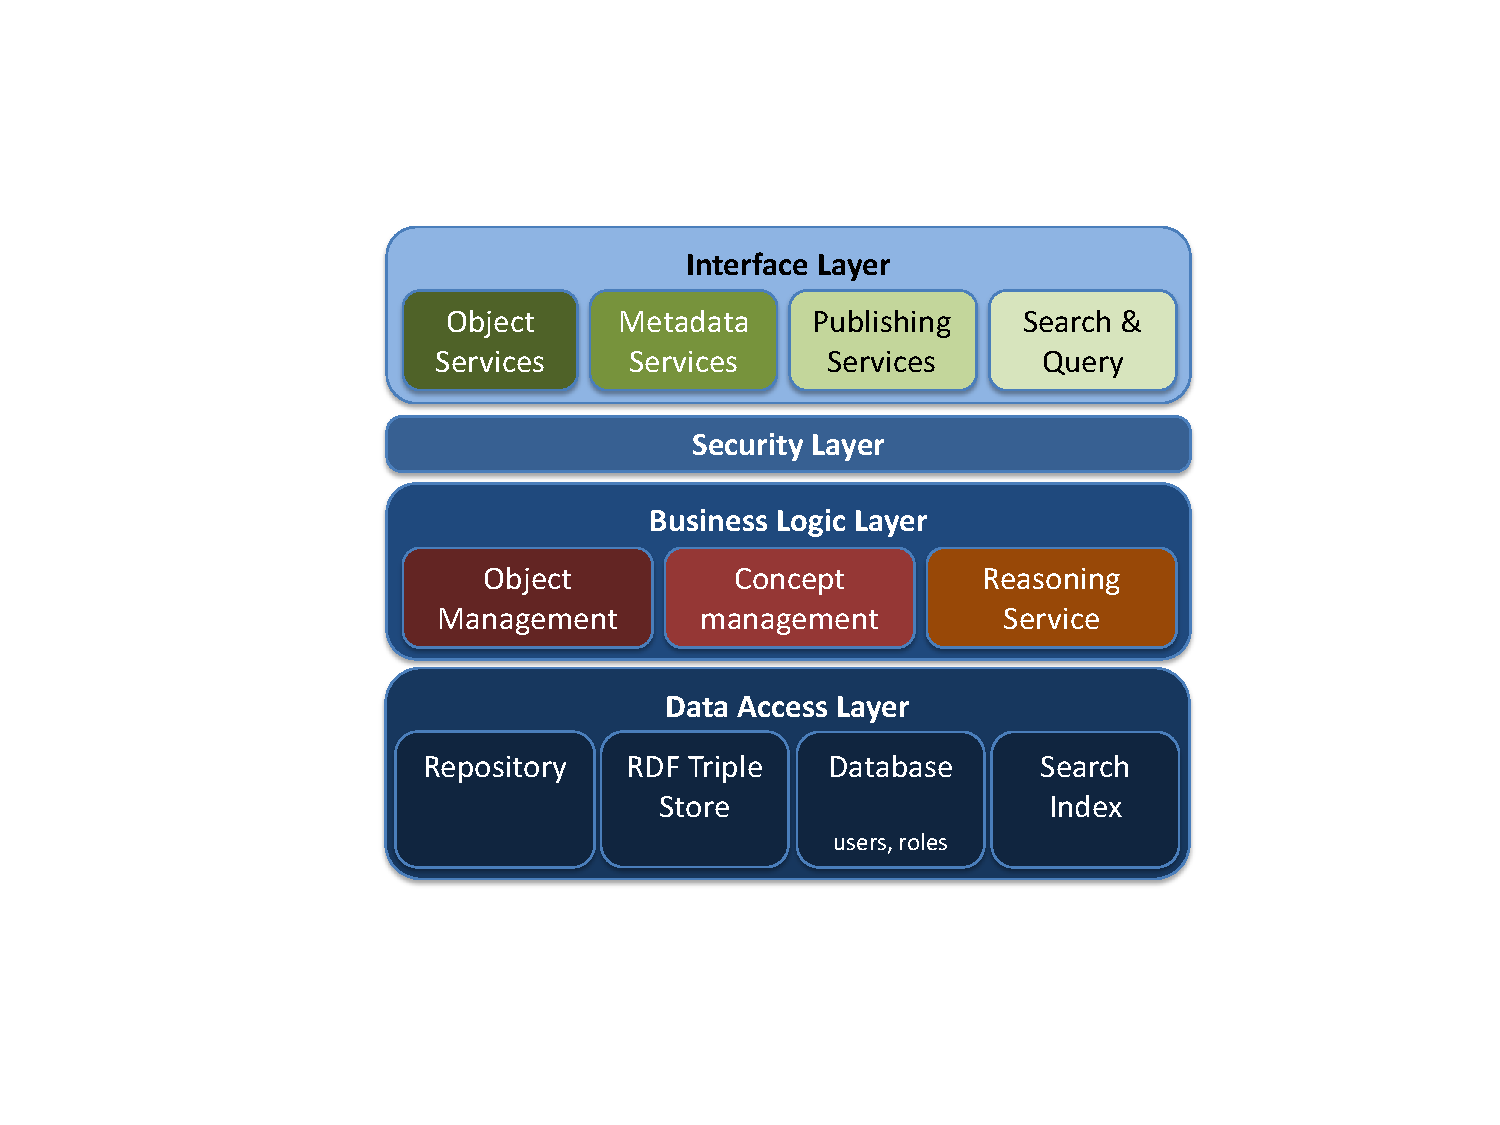
\includegraphics[trim = 60mm 30mm 50mm 38mm, clip,height=55mm]{architecture.pdf}
\vspace{-16pt} \caption{A high-level depiction of components in the
ontology-driven architecture.}\label{fig:arch}
\end{figure}

The high-level design of ontology-centric architecture takes a modular
and layered approach, as can be seen in Figure~\ref{fig:arch}. At the
foundation is the \textbf{data access layer}, consisting of an
underlying repository system, an RDF triple store, an in-house database
that stores essential information and a full-text search engine. This
layer is responsible for low-level tasks when the creation,
modification and deletion of concepts and objects occur. The
\textbf{business logic layer} in the middle is responsible for managing
concepts and objects, such as versioning, object conversion and
integrity validation. The \textbf{security layer} controls access
(authentication and authorization) to concepts and objects and guards
all operations on them.
%In this architecture, authorization is based on user attributes, which have two dimensions.
%Firstly, each user has a system-wide role, such as registered user or
%system administrator, which is used to determine access rights across
%the system. Secondly, a project-wide role, such as project
%administrator and project observer, can be assigned to a user so that
%he can have project-specific access rights.
At the top of the stack is the \textbf{interface layer}, where the data
management system can be accessed using a number of interfaces such as
a Web browser or API calls.

In developing the ontology-centric architecture, the following design
decisions have been made to balance expressivity, flexibility and
conceptual clarity. These decisions have also been based on a survey of
user requirements from scientists within a range of research
organizations including the Australian Plant Phenomics Facility (APPF)
as well as the Institute of Molecular Biology (IMB), Queensland Brain
Institute (QBI) and Australian Institute of Bioengineering \&
Nanotechnology (AIBN), working on collaborative research projects that
involve large scale data and distributed teams:

\begin{itemize}
\item There is a top-level domain concept, called Project , under which
other concepts (such as Investigation and Material) reside in a
hierarchical manner.

\item Access control (authorization) is defined on the Project level but
not on an individual object level, i.e., a given user will have the
same access rights for all objects within a given project.

\item Within a Project hierarchy, objects are in a parent-child
relationship in a tree structure such that each child can only have one
parent. This ensures that access rights are properly propagated from
parent to child and there is no chance of confusion.

\item Additionally, inter-object, many-to-many reference relationships
can be defined to enhance flexibility of the architecture as it allows
arbitrary links between objects to be established.

\item Objects cannot be shared across Projects. Instead, objects must be
copied from one project and pasted into another one. Such a rule
simplifies object management with the elimination of possible
side-effects caused by sharing object between projects.

\item There should be no interference between different versions of a
given concept and between objects that are instances of different
concept versions.
\end{itemize}

\section{Ontology-based Domain Modeling}\label{sec:ont}
As we emphasized previously, the domain model should be flexible enough
to accommodate the rapid changes and dynamic nature of scientific
research. In this section, we present the base ontology and the roles
it plays in the ontology-centric architecture. It should be noted that
the architecture proposed here is domain-independent and it can be
applied to any scientific discipline that shares a similar high-level
domain model.

Note that concepts in the ontologies presented here are models of entities
(activities and objects) in scientific investigations: they define the logical
structure of investigations - objects in an investigation and logic relationship 
between these objects. 
In a sense, the ontologies serve as a data model of the investigations in 
the scientific domain for which the data management system is developed.
In other words, the ontologies are used as a model for the data management 
system implementation.

\subsection{The Base Domain Ontology}
Inspired by FuGe~\cite{citeulike:1756058} and
OBI\footnote{\url{http://purl.obolibrary.org/obo/obi}}, we created the
base domain ontology in OWL to define essential domain concepts, their
attributes and inter-relationships in an object-oriented fashion. As
stated in the previous section, domain concepts will be modeled as OWL
classes; relationships between concepts and object attributes will be
modeled as OWL object and datatype properties. Concrete objects will be
modeled as OWL individuals.

\vspace{-16pt}
\begin{figure}[htb]
\centering
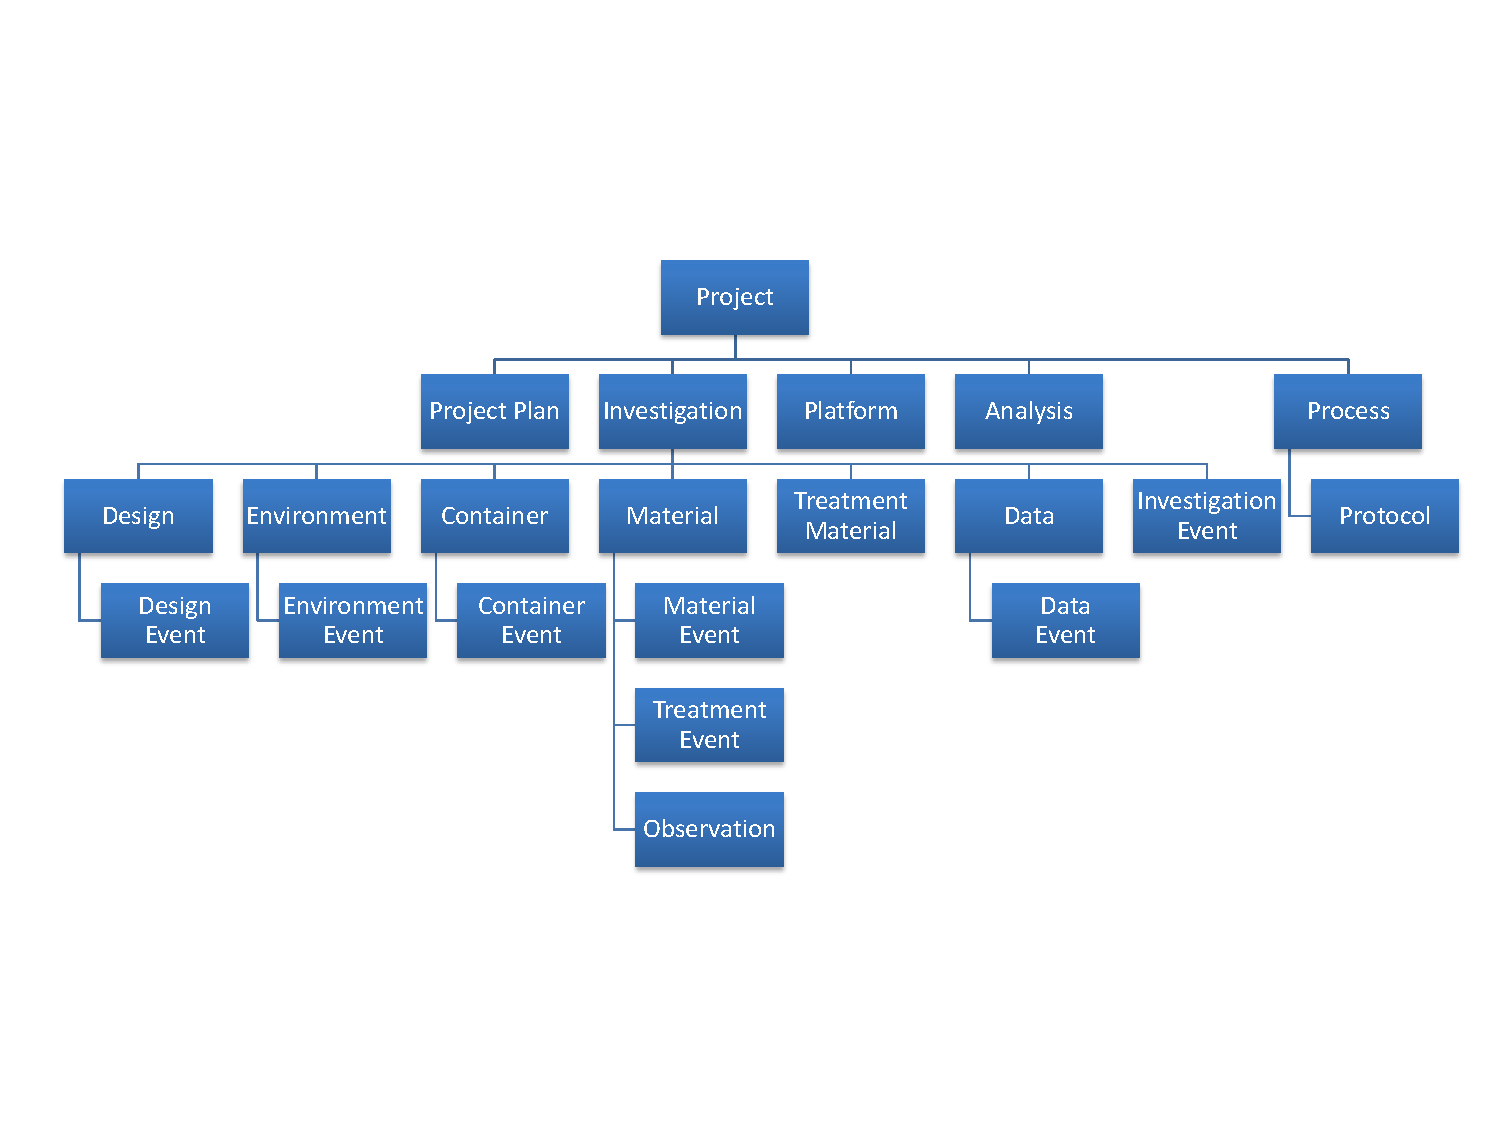
\includegraphics[trim = 5mm 30mm 5mm 46mm, clip,height=50mm]{ont_high.pdf}
\vspace{-16pt} \caption{Main concepts in the base
ontology in the parent-child relationship \emph{contains}.}\label{fig:ont_high}
\end{figure}

\vspace{-16pt}
For an overview, inter-relationships of some of the domain concepts in
this ontology are shown in Figure~\ref{fig:ont_high}. It is worthing 
pointing out that concepts in this figure are shown in the logical 
hierarchy but not the inheritance hierarchy: it describes the structure 
of a scientific investigation and
how different activities/objects in it are related to each other.
For brevity reasons, OWL object properties and cross
references between classes are not shown. We also defined the following
design principles for the domain ontology. 

\begin{itemize}
\item All essential domain concepts are modeled as sub-classes of an
abstract top-level OWL class \emph{PODDConcept} that captures common
attributes and relationships.

\item All relationships between domain concepts are captured by domain
properties, which can be further divided into two property hierarchies,
one for parent-child relationships and the other for reference
relation-ships. Each of the two hierarchies have an abstract top-level
property, called \emph{contains} and \emph{refersTo}, respectively.

\item All parent-child relationships are modeled in a property hierarchy
as sub-properties of the abstract property \emph{contains}, and all
reference relationships are modeled in another property hierarchy as
sub-properties of the abstract property \emph{refersTo}.

\item For each domain concept \emph{C}, one property is defined in each of the
above hierarchies with its range defined to be \emph{C}. The domains of
such properties are not specified so that they can be used by any
applicable domain concept to establish a relationship between them.

\item Class attributes are modeled using OWL restrictions.

\item Essential domain concepts can be sub-classed to provide more
specialized and refined information.

\item To ensure that each object can have at most one parent object, the
inverse property of \emph{contains}, \emph{isContainedBy}, is defined
so that a max cardinality restriction can be added to the top-level
concept \emph{PODDConcept} to enforce it.
\end{itemize}

The definitions of some top-level constructs are summarized in
Figure~\ref{fig:top}, in OWL DL syntax~\cite{hoph03a}.

\vspace{-16pt}
{\small
\begin{figure}
\begin{align*}
& PODDConcept \sqsubseteq \top && \top \sqsubseteq \forall contains.PODDConcept\\
& isContainedBy \sqsubseteq (^- contains) && PODDConcept \sqsubseteq \leq 1~ isContainedBy\\
& \top \sqsubseteq refersTo.PODDConcept &&
\end{align*}

\vspace{-8pt}
\caption{Top-level ontology constructs in the PODD
ontology}\label{fig:top}
\end{figure}}

\vspace{-12pt}
In our model, we use OWL properties to model object attributes. When
the possible values of a particular attribute can be enumerated, such
as project status (\emph{active}, \emph{inactive} and
\emph{completed}), an enumerated OWL class is used to represent all the
values. When an attribute represents a grouping of some values, such as
accessions, where an accession has a source and a number, an OWL class
is also defined to represent the grouping. In this case, auxiliary OWL
properties are defined to project out specific values in the grouping.
In all other cases, attributes are modeled using datatypes.

Figure~\ref{fig:project_owl} shows the partial definition of the OWL
class $Project$. Restriction (\ref{for:hasPlan}), for example, states
that any $Project$ instance must have exactly one $ProjectPlan$
(through the predicate $hasProjectPlan$, the range of which is
$ProjectPlan$). The other 3 restrictions are similarly defined.

\vspace{-16pt}
\begin{figure}[htb]
\centering \small
\begin{align}
Project \sqsubseteq~ &=~ 1~ hasProjectPlan~ \sqcap \label{for:hasPlan}\\
        \sqsubseteq~ &\geq~ 1~ hasInvestigation~ \sqcap \\
        \sqsubseteq~ &=~ 1~ hasStartDate~ \sqcap\\
        \sqsubseteq~ &\leq~ 1~ hasPublicationDate
\end{align}
\vspace{-16pt} \caption{Partial OWL Definition for the Project
concept.}\label{fig:project_owl}
\end{figure}

\vspace{-24pt}
\subsection{Roles of Domain Ontologies in Object Life Cycle}
The base ontology defines essential concepts independent of the domain.
Domain-specific knowledge can be incorporated by extending the base
ontology for discipline-specific systems.

As stated in Section~\ref{sec:intro}, the ontology-based domain model
is at the center of the whole life cycle of objects. In this
subsection, we briefly describe the roles that the domain ontologies
perform at various stages of the object life cycle.

\begin{description}
\item[Ingestion]
When an object is created, its definition is expressed in
ontological terms. Such definitions will be used to (a) guide the
rendering of object creation interfaces and (b) validate the attributes
and inter-object relationships the user has entered before the object
is ingested. When an object is ingested, its definitions are stored as
RDF assertions.

\item[Retrieval \& update] When an object is retrieved from the
repository, its attributes and inter-object relations are retrieved
from its RDF assertions, which are used to drive the on-screen
rendering. When any value is updated, it is validated and updated in
this object's RDF assertions.

\item[Query \& search] An object's assertions will be stored in an RDF
triple store, which can be queried using SPARQL. Similarly, ontological
definitions are indexed to provide functionalities such as full-text
search and faceted browsing.

\item[Publication \& export] When an object is published or exported, its
metadata, in RDF, will be retrieved and exported.
\end{description}

\section{The PODD Data Management System}\label{sec:podd}
Based on the ontology-centric architecture presented in
Section~\ref{sec:arch} and the base ontology presented in
Section~\ref{sec:ont} we implemented the PODD data management system -
with the aim being to meet the data management challenges faced by the
Australian phenomics research community.

To describe domain knowledge in phenomics, we extend the base ontology
by defining additional concepts including \emph{Genotype}, \emph{Gene},
\emph{Phenotype} and \emph{Sequence} as subclasses of
\emph{PODDConcept}. Additional OWL object and datatype properties are
also defined to model the attributes and relationships of these
concepts, as shown in Figure~\ref{fig:podd_high}. Note that
\emph{Phenotype} is a subclass of \emph{Observation}.

\begin{figure}[htb]
\centering
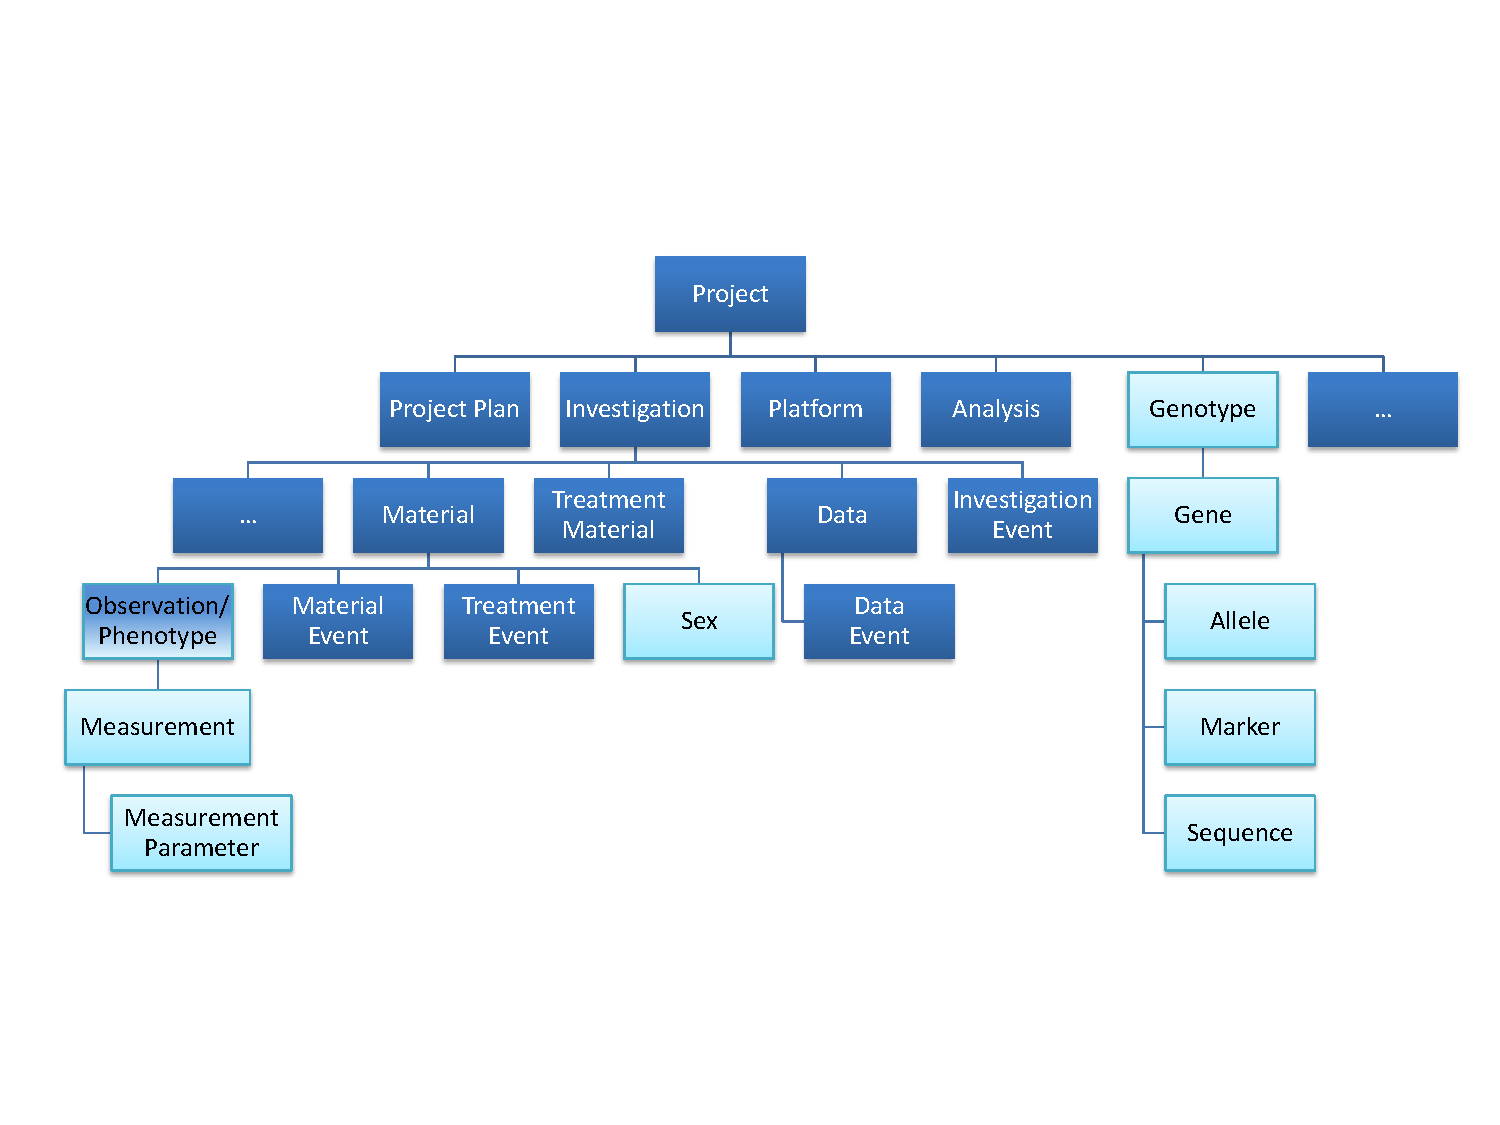
\includegraphics[trim = 5mm 30mm 5mm 46mm, clip,height=50mm]{ont_podd.pdf}
\vspace{-16pt} \caption{Extended Domain Ontology for
phenomics.}\label{fig:podd_high}
\end{figure}

Figure~\ref{fig:phe_ont} shows some new definitions in the domain
ontology. Note that the last two definitions
integrate the new definitions with those in the base ontology.

Also note that the concepts defined in the PODD ontologies do not
necessarily represent real-world entities/reality. For example, the OWL class
\emph{Gene} does not intend to be a class that describes genes
in general. Rather, it is used to describe genes that are observed/involved
in scientific investigations.

\vspace{-16pt}
{\small
\begin{figure}[htb]
\centering
\begin{minipage}[t]{.55\linewidth}
\centering
\begin{align*}
Genotype &\sqsubseteq~ PODDConcept\label{for:hasPlan}\\
         &\sqsubseteq~ \forall hasGene.Gene\\
         &\sqsubseteq~ \leq~ 1~ hasEcotype\\
         &\sqsubseteq~ \leq~ 1~ hasSubspecies\\
         &\cdots\\
Project  & \sqsubseteq \forall hasGenotype.Genotype\\
Material & \sqsubseteq \forall hasPhenotype.Phenotype\\
         & \sqsubseteq \forall refersToGenotype.Genotype
\end{align*}
\end{minipage}
\begin{minipage}[t]{.4\linewidth}
\centering
\begin{align*}
Gene & \sqsubseteq~ PODDConcept\\
     & \sqsubseteq~ \forall hasSequence.Sequence\\
     & \sqsubseteq~ \leq~ 1~ hasAlias\\
     & \sqsubseteq~ \leq~ 1~ hasChromosome\\
     & \cdots
\end{align*}
\end{minipage}

\vspace{-4pt}
\caption{Domain-specific OWL definitions.}\label{fig:phe_ont}
\end{figure}
}

\vspace{-12pt}
In developing the PODD system, we chose to employ a number of mature
technologies. (1) We use Fedora Commons for the storage and retrieval
of domain objects. Together with raw data files, the OWL (for concepts)
and RDF (for objects) definitions of each concept and object are stored
in a versioned datastream PODD, which is used by the PODD system in
various tasks such as object creation, rendering, validation, update
and visualization. (2) We incorporate
the Sesame triple store\footnote{\url{http://www.openrdf.org/}} to
support complex query answering using SPARQL. Sesame contexts are used
to give scope to the RDF triples for each domain object. As described
in Section~\ref{sec:arch}, access control needs to be enforced on a per
project level. Similarly, it also needs to be enforced on query
answering in the triple store. By identifying triples of individual
objects, we are able to control contexts a user can access through
query expansion. (3) Lastly, we use the Lucene and Solr open-source search
engine platform\footnote{\url{http://lucene.apache.org/}} to provide
full-text search and faceted browsing capabilities. Similar to the
structure of the Sesame triple store, there is a one-to-one
correspondence between domain objects in the repository and the Solr
documents, the logical indexing units.

\vspace{-8pt}
\begin{figure}[htb]
\centering
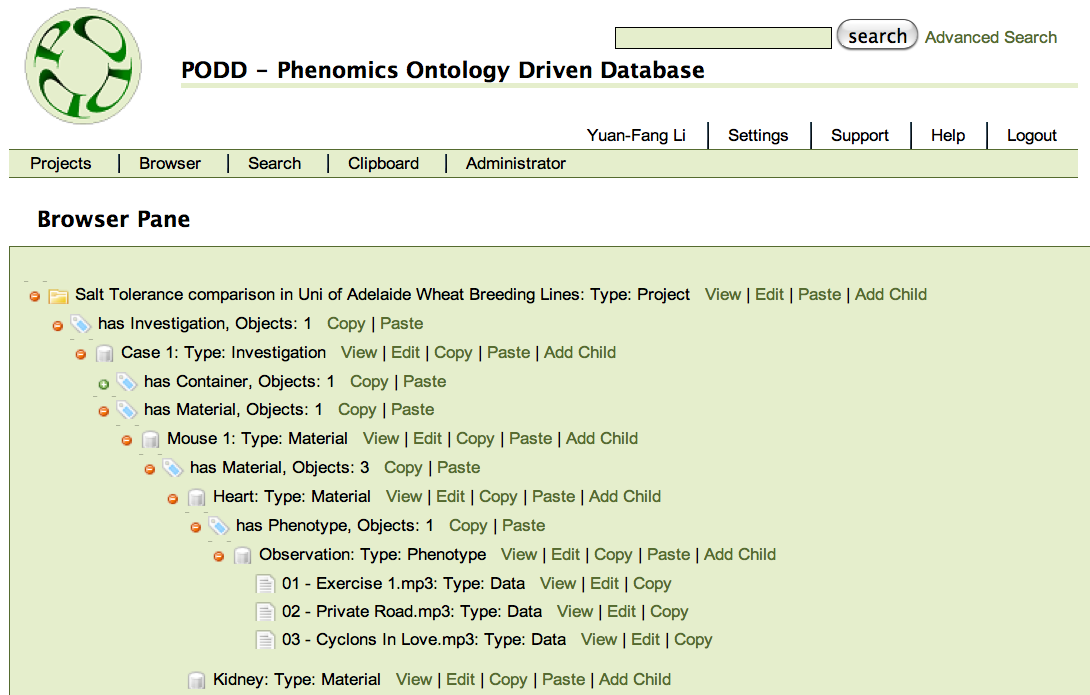
\includegraphics[trim = 5mm 0mm 5mm 0mm, clip,height=76mm]{browser.png}
\vspace{-8pt} \caption{The browser view of a plant project in the PODD
repository.}\label{fig:browser}
\end{figure}

\vspace{-8pt}
Although the architecture and the system are based on ontologies, the
interface is designed to hide ontology-related complexity from the user
and present information in an easy to use manner for all repository
functions. For example, Figure~\ref{fig:browser} shows the browser view
of a plant phenomics project that investigates salt tolerance of wheat. 
In this view, the objects are shown in a tree-like structure by following
property assertions of subproperties of contains defined in  the base
and domain ontologies.

We have started to deploy the PODD system in Australian phenomics
research centers including APPF and APN and begun engaging users in the
evaluation of the performance, flexibility, usability and scalability
of the system. User feedback to date has shown that the system is
intuitive and efficient.

\section{Conclusion}\label{sec:concl}
In summary, our contribution to scientific data management is
three-fold: firstly, the proposal of the ontology-centric architecture
for developing data management systems; secondly, the development of a
base ontology that defines essential domain knowledge; and thirdly, the
development of the PODD data management system (based on both existing
and new technologies) that validates the feasibility of the proposed
approach.

We have identified a number of future work directions that we would
like to pursue. Firstly, we will investigate integration with existing
domain ontologies such as the Gene Ontology and the Plant Ontology. One
possibility would be to use terms defined in these ontologies to
annotate metadata objects. Secondly, we would like to investigate the
generalization of the ontology-centric approach so that it can be
applied to other areas such as workflow management systems. Thirdly, we
will continue the development of the PODD system to provide additional
functionalities such as data visualization, automated data integration
and Linked Data-style data discovery and publication.

%\section*{Acknowledgment}
%The authors wish to acknowledge the support of the National eResearch
%Architecture Taskforce (NeAT) and the Integrated Biological Sciences
%Steering Committee (IBSSC) Australia. The authors wish to thank Dr
%Xavier Sirault, Dr. Kai Xu and Mr. Philip Wu for the discussion and
%assistance in the development of the domain ontology and the PODD
%system.

\bibliography{all}
\bibliographystyle{abbrv}
\end{document}
